\documentclass[a4paper,12pt]{report}
\usepackage{color}
\usepackage{hyperref}
\hypersetup{
    colorlinks,
    citecolor=black,
    filecolor=black,
    linkcolor=black,
    urlcolor=blue
}
\setcounter{secnumdepth}{0}
\usepackage{graphicx}
\usepackage[font=small,labelfont=bf]{caption}
\usepackage{epstopdf}
\epstopdfsetup{outdir=./}	
\usepackage{amsmath}
\usepackage[table,xcdraw]{xcolor}
\usepackage{amssymb}
\usepackage{listings}
\definecolor{anti-flashwhite}{rgb}{0.95, 0.95, 0.96}
\lstset{
	language=C++,
    basicstyle=\ttfamily,
    keywordstyle=\color{blue}\ttfamily,
    stringstyle=\color{red}\ttfamily,
	commentstyle=\color{green}\ttfamily,
    morecomment=[l][\color{magenta}]{\#},
    backgroundcolor=\color{anti-flashwhite}
}
\begin{document}
\title{
\textbf{Compilers II: CS3423}\\~\\
\begin{large}
\textbf{Mini Assignment II\\~Introduction to Polly}\\~\\~\\
\end{large}
\begin{large}
\textbf{Assignment Report}
\end{large}
}
\author{\textbf{Sagar Jain - CS17BTECH11034}\\}
\maketitle
\begin{large}
\tableofcontents
\end{large}
\newpage
\section{Architecture and Intuitive Understanding of Polly}
\subsection{What is Polly to LLVM?}
In the simplest possible words, \textbf{Polly is a loop optimizer for LLVM}. Polly fits into the LLVM pass pipeline. LLVM basically has three phases in the pass pipeline:
\begin{enumerate}
\item Canonicalization
\item Inliner cycle
\begin{enumerate}
\item Scalar Simplification
\item Simple Loop Optimizations
\item Inliner
\end{enumerate}
\item Target Specialization
Polly can conceptually be run at three different positions in the pass pipeline, but mostly it is run as (1) an early optimizer before the standard LLVM pass pipeline or (2) as a later optimizer as part of the target specialization sequence.
\end{enumerate}
\begin{center}
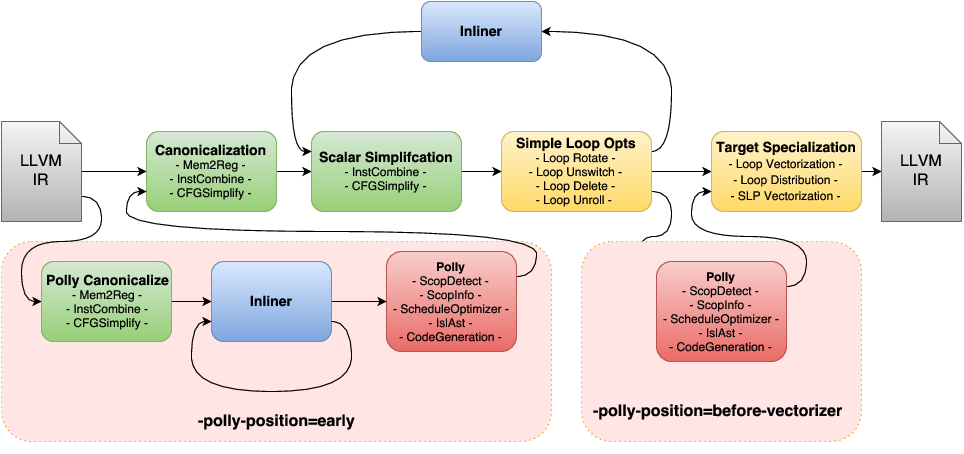
\includegraphics[scale=0.45]{llvm-passes.png}
\captionof{figure}{Image from \href{https://polly.llvm.org/docs/Architecture.html\#polly-in-the-llvm-pass-pipeline}{here}}~\\
\end{center}
\subsection{Understandig of the Polyhedral Model}
The following is a my idea of how a polyhedral model works. First we need to understant that a loop, during execution can be represented in an alternate way. Each instruction loop should be considered as a different instance in every iteration. This way we have a set of \textbf{instruction instances}. Instruction not in loops would, intutively, have only single instances in normal circumstances.\\
Now that we have a set of instruction instances, we need to execute them. The ordering of this execution is where polly comes in. \textbf{Suppose we make a graph with all the instruction instances as nodes and an incoming edge into nodes from all the nodes which need to be executed before it}. We would now have something like this:
\begin{center}
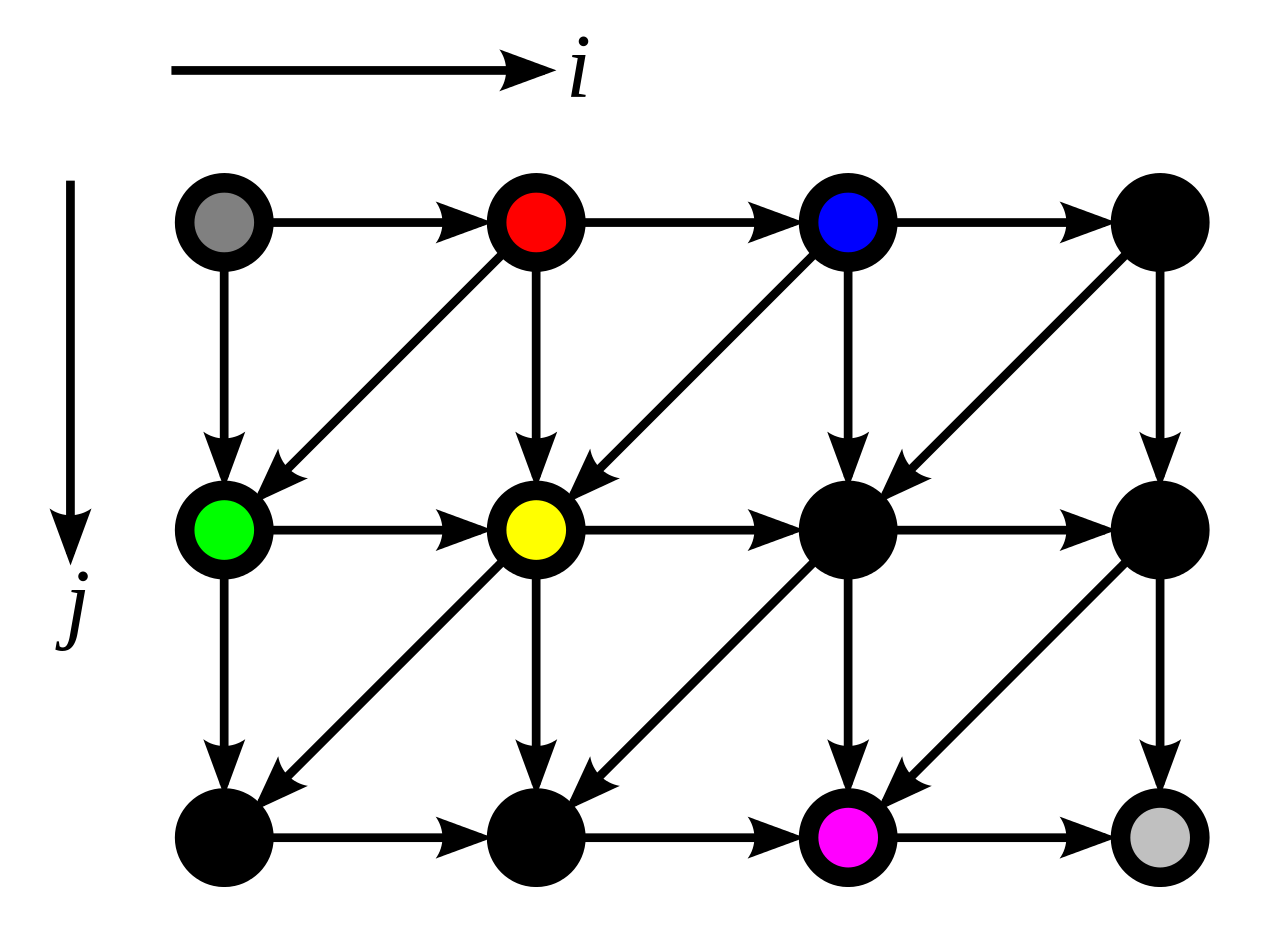
\includegraphics[scale=0.13]{polyi.png}
\captionof{figure}{Image from \href{https://en.wikipedia.org/wiki/Polytope\_model}{here}}
\end{center}
All we know here is that an instruction must not be executed before all the instruction it depends on are executed. Also this representation ends up looking like a polyhedral in most cases (rectangle in this case) and that's where the name comes from. Polly finds the best possible \textbf{"skewing"} of this polyhedral such that the most number of instructions can be  executed parallely, minimising time. This seems to be a complex ILP problem. The result for the current case would something like the following.
\begin{center}
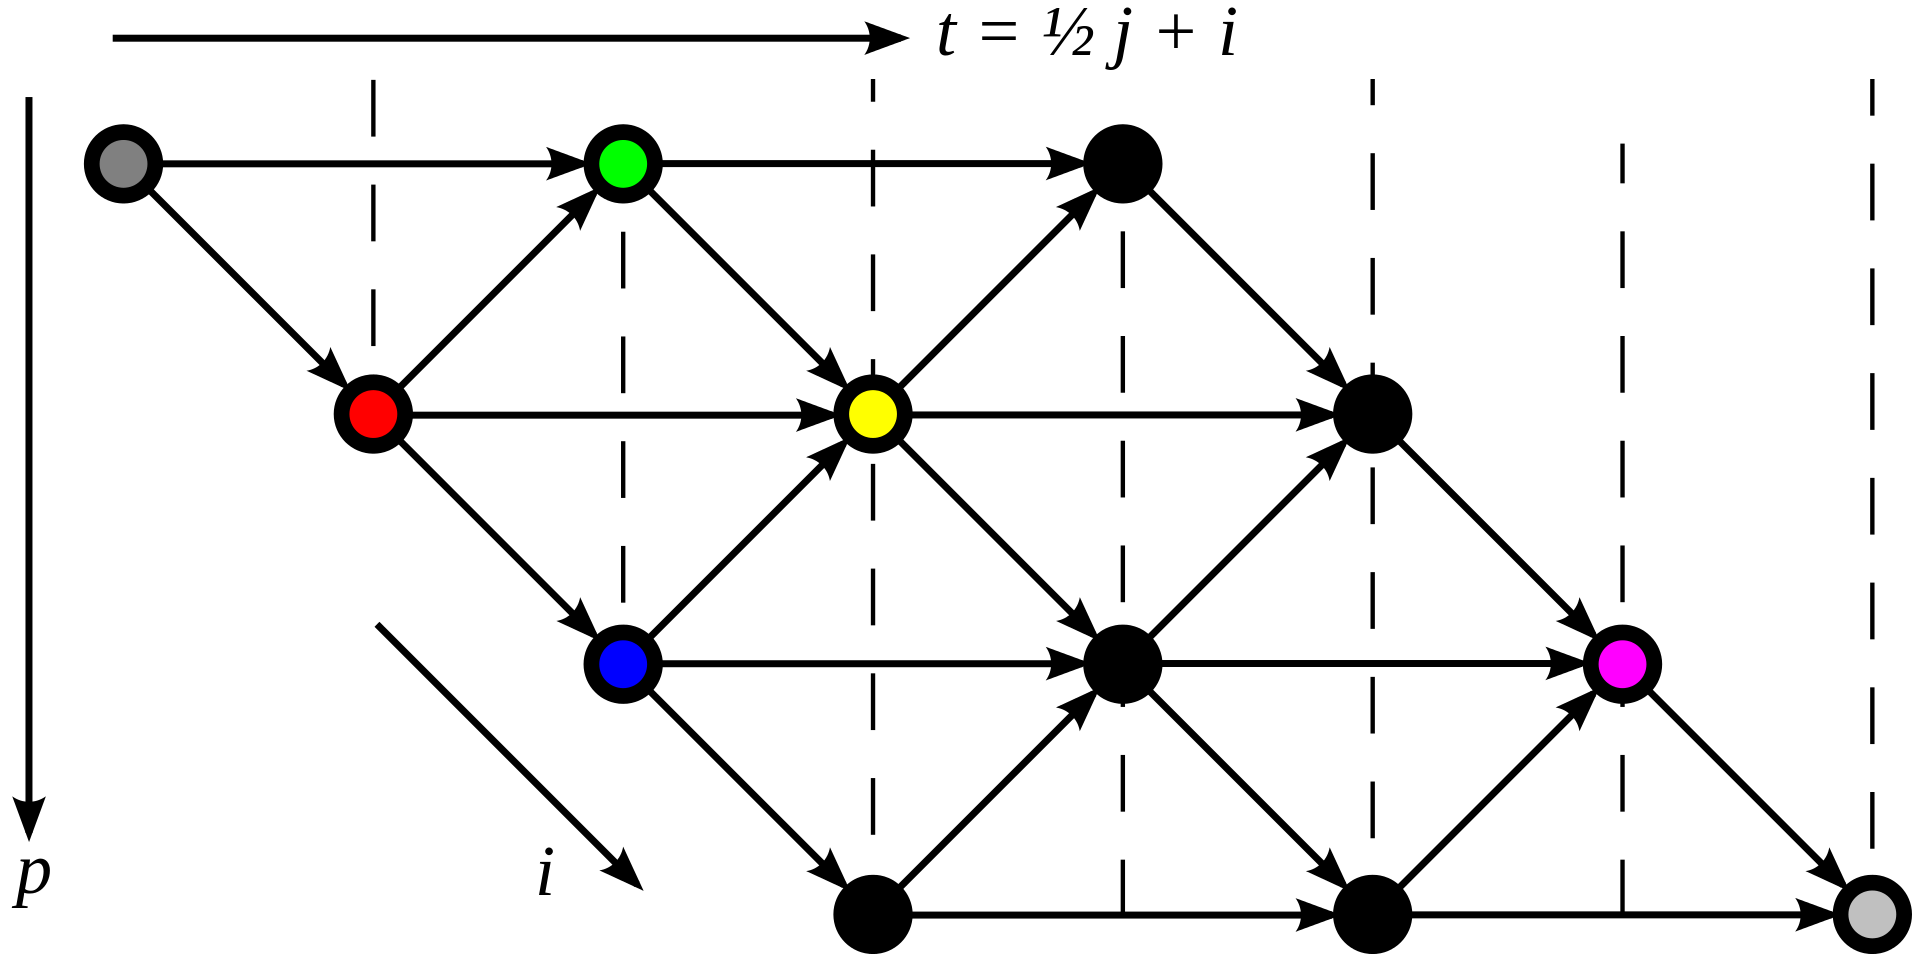
\includegraphics[scale=0.13]{polyf.png}
\captionof{figure}{Image from \href{https://en.wikipedia.org/wiki/Polytope\_model}{here}}
\end{center}
\newpage
\section{Results}
The following are the results for the file matmul.c from \href{https://raw.githubusercontent.com/llvm-mirror/polly/master/docs/experiments/matmul/matmul.c}{here}. \\\\
\begin{tabular}{|l|l|}
\hline
Compile Options & Time Taken \\ \hline
clang -O3 & 27.95s \\ \hline
gcc & 84.90s \\ \hline
gcc -O3 & 6.06s \\ \hline
clang -O3 -mllvm -polly & 0.39s \\ \hline
\end{tabular}\\\\\\
These results seem almost too good to believe, this shows the great utility of polyhedral compilation. We get around 21769\% improvement over normal gcc compilation and 1550\% over gcc with O3, this is phenomenal by any standards.  
\section{Analysis of Transformed Code \& Trying Other Polly Options}
I tried the following optimisations with polly:
\begin{enumerate}
\item \texttt{polly-vectorizer=stripmine}
\item \texttt{polly-parallel-force}
\item \texttt{polly-tiling}
\end{enumerate}
The following are the most important characteristics of the polly-generated IR I noticed:
\begin{enumerate}
\item Firstly, the generated IR is much bigger interms of code-size than the normal IR (without polly) for the same file.
\item In every loop there are a lot of constant variables declared in the header, these are begin used as offsets \textbf{getelementptr}.
\item SCEV is being used extensively in the IR. This makes sense since SCEV is important to get bounds and steps and these are used by the polyhedral model to compute how to manipulate i.e. skew the execution process.
\item Another important thing I noticed is that most of the scev computation happens in the header of loops, this happens because once the loops are skewed their initial conditions, steps and bounds are altered and need the loop conditions need to be computed at every iteration.
\end{enumerate}
\newpage
\section{SCoPs and Dependencies}
SCoP stands for Static Control Parts. Static control essentially means control flow within the loop only depends on the loop iterators only. An important part of the polyhedral model is to determine if the schedule computed by it is \textbf{legal}. This, quite obviously depends on the \textbf{dependecies} between instructions and instruction instances. In the \texttt{matmul.c} file the main function has the following SCoPs:
\begin{center}
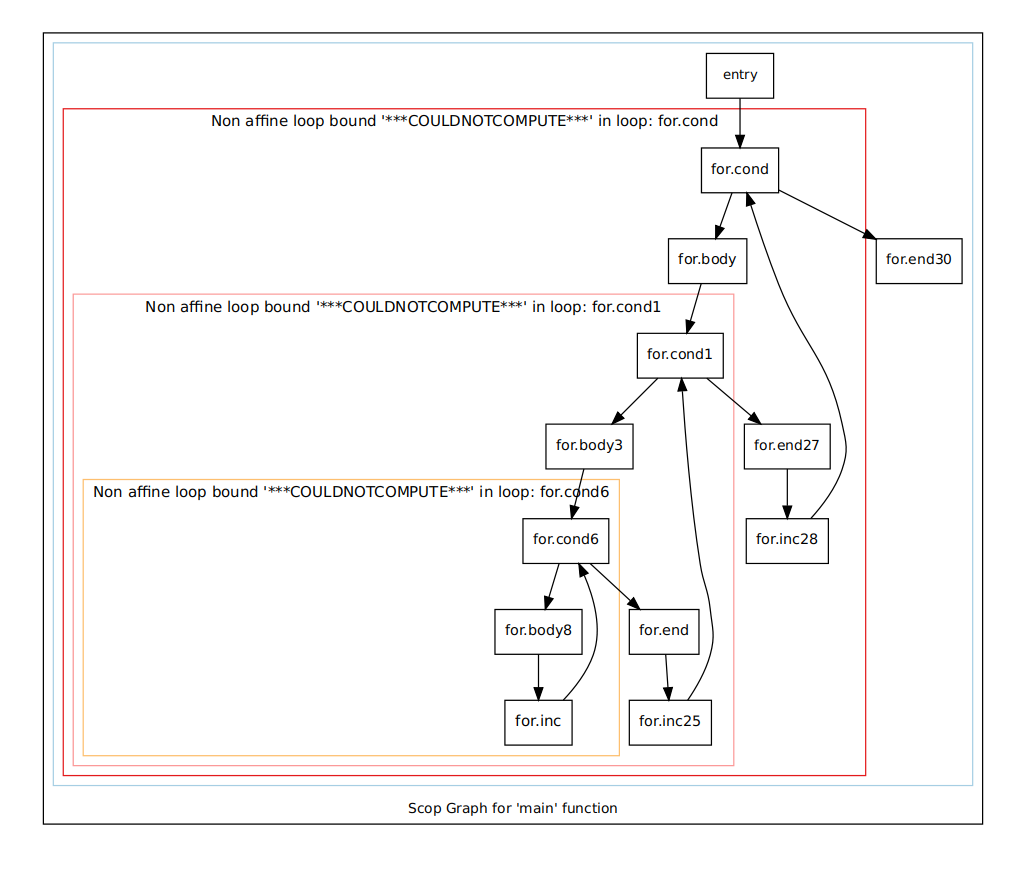
\includegraphics[scale=0.40]{scop.png}
\captionof{figure}{}
\end{center}
The SCoP and static reference assumptions assumption is very important to get an exact set of instances in dependence. One can even get the dependences for SCoPs using:\\
\texttt{opt -polly-dependences -analyze matmul.preopt.ll -polly-process-unprofitable}
\newpage
\section{References}
\begin{itemize}
\item \href{https://wiki.aalto.fi/display/t1065450/Polyhedral+optimizations+with+LLVM}{https://wiki.aalto.fi/display/t1065450/Polyhedral+optimizations+with+LLVM}
\item \href{http://polly.llvm.org/docs/HowToManuallyUseTheIndividualPiecesOfPolly.html}{http://polly.llvm.org/docs/HowToManuallyUseTheIndividualPiecesOfPolly.html}
\item \href{http://polly.llvm.org/docs/UsingPollyWithClang.html}{http://polly.llvm.org/docs/UsingPollyWithClang.html}
\item \href{http://www.es.ele.tue.nl/~rjordans/5LIM0/10-polyhedral-model.pdf}{http://www.es.ele.tue.nl/~rjordans/5LIM0/10-polyhedral-model.pdf}
\end{itemize}
\end{document}